\documentclass[10pt]{beamer}
\usepackage[utf8]{inputenc}
\usepackage{graphicx}
\usepackage{mathtools}
\usetheme{CambridgeUS}
\usecolortheme{dolphin}
\usepackage{listings}

% Set up hyperref once and configure colors
\usepackage{hyperref}
\hypersetup{
    colorlinks=true,
    linkcolor=blue,
    linktocpage=true
}

% Custom colors
\definecolor{myNewColorA}{RGB}{118,193,188}
\definecolor{myNewColorB}{RGB}{106,172,150}
\definecolor{myNewColorC}{RGB}{94,150,218}
\setbeamercolor*{palette primary}{bg=myNewColorC}
\setbeamercolor*{palette secondary}{bg=myNewColorB, fg=white}
\setbeamercolor*{palette tertiary}{bg=myNewColorA, fg=white}
\setbeamercolor*{titlelike}{fg=myNewColorA}
\setbeamercolor*{title}{bg=myNewColorA, fg=white}
\setbeamercolor*{item}{fg=myNewColorA}
\setbeamercolor*{caption name}{fg=myNewColorA}
\usefonttheme{professionalfonts}

\titlegraphic{
\includegraphics[height=1.5cm]{../CommonFigures/Universidad_Panamericana-logo.jpg}}

\setbeamerfont{title}{size=\large}
\setbeamerfont{subtitle}{size=\small}
\setbeamerfont{author}{size=\small}
\setbeamerfont{date}{size=\small}
\setbeamerfont{institute}{size=\small}
\title[Universidad Panamericana]{}
\subtitle{FreeRTOS Architecture Part 1}
\author[]{Name}
\institute[ltonix@up.edu.mx]{Universidad Panamericana}
\date[Presentation \today]{Presentation \today}

\AtBeginSection[]{
  \begin{frame}
  \vfill
  \centering
  \begin{beamercolorbox}[sep=8pt,center,shadow=true,rounded=true]{title}
    \usebeamerfont{title}\insertsectionhead\par%
  \end{beamercolorbox}
  \vfill
  \end{frame}
}

\setbeamercolor{block title}{bg=myNewColorA, fg=black} % Background and foreground colors for the block title
\setbeamercolor{block body}{bg=myNewColorC, fg=black} % Background and foreground colors for the block body

% Setup listings
\lstset{
  basicstyle=\ttfamily\small,
  keywordstyle=\color{blue},
  commentstyle=\color{green},
  stringstyle=\color{red},
  backgroundcolor=\color{gray!10},
  frame=single,
  language=C++,
  breaklines=true,
  showspaces=false,
  showstringspaces=false
}


\begin{document}

\frame{\titlepage}
\begin{frame}
\frametitle{Contents}
\tableofcontents
\end{frame}



\section{Defensive Programmig}

\begin{frame}{Defensive Programmig. Expect the unexpected}
  
Defensive programming is a bit like always wearing a full suit of armor. It’s about preparing for the worst while hoping for the best, much like someone living in a zombie apocalypse with a bunker full of canned goods. In this approach, every function call is a potential trick, every user input a Trojan horse, and paranoia isn’t just recommended, it’s required!

  \begin{figure}[h]
    \centering
    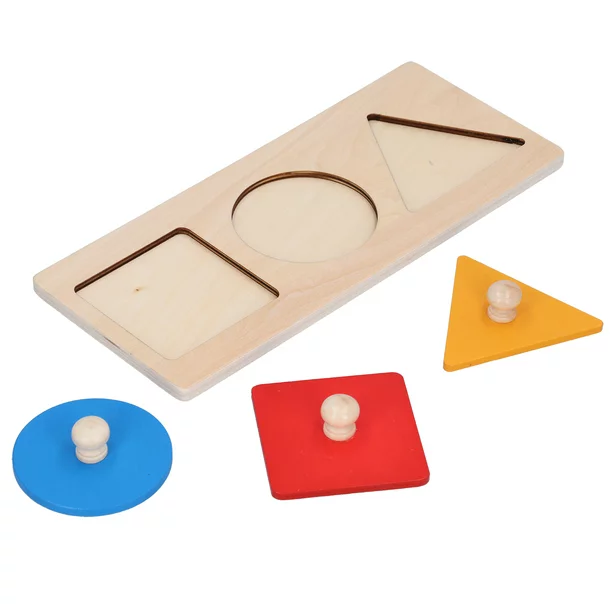
\includegraphics[width=0.25\textwidth]{figures/BadDummpyProof.png}
    \label{fig:BadDummpyProof}
  \end{figure}


\end{frame}

\begin{frame}{Defensive Programmig. Expect the unexpected}
  Good Practice
  \begin{figure}[h]
    \centering
    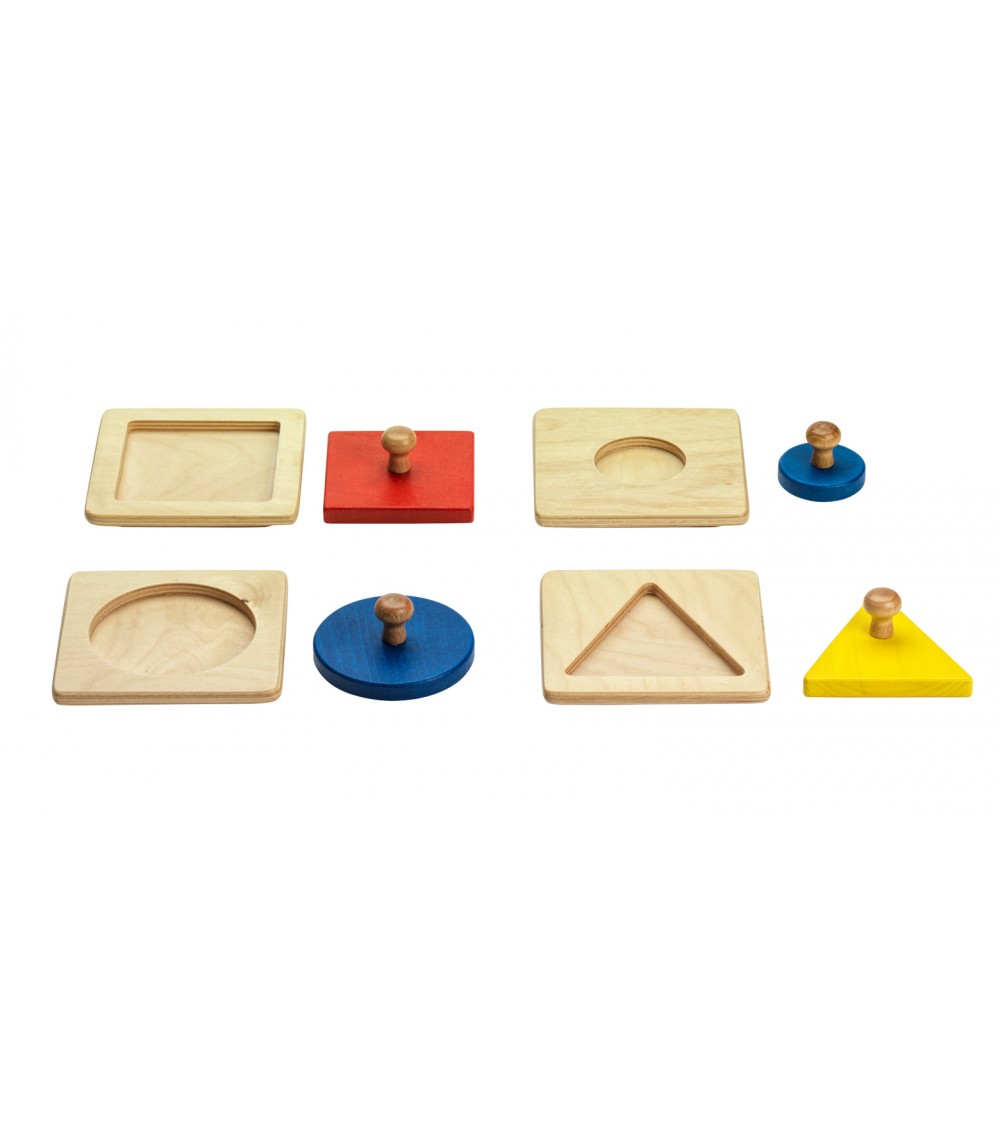
\includegraphics[width=0.5\textwidth]{figures/GoodDummyProof.png}
    \label{fig:BadDummpyProof}
  \end{figure}
\end{frame}
\begin{frame}{Defensive Programmig. Expect the unexpected}
  \begin{itemize}
    \item Thats why is a good practice to use C++
    \item C++ has \href{https://en.cppreference.com/w/cpp/language/Zero-overhead_principle}{Zero Over Head Principle}.
    \item Learn C++ and you can find a better job,and just add a plus to your resume. 
  \end{itemize}
\end{frame}
\subsection{Using const for Safety}
\begin{frame}{Using const for Safety}
  \begin{itemize}
    \item const keyword: ensures variables are not modified after initialization.
    \item Use const to protect function parameters, class members, and pointers.
    \item Example: void process(const Data\& data); guarantees data remains unchanged.
    \item This is used for read only variables.
  \end{itemize}
\end{frame}

\begin{frame}[fragile]{Using const in C++}
  \begin{lstlisting}
    class Person {
      public:
          string name;
          int age;
          Person(string n, int a) : name(n), age(a) {}
      
          void print() const {
              cout << "Name: " << name << ", Age: " << age << endl;
          }
      };
      
      void displayPerson(const Person& p) {
          p.print();
      }
  \end{lstlisting}
\end{frame}


\section{Memory Managment}

\subsection{Memory Hierarchy}
\begin{frame}{Memory Hierarchy: A Light-Hearted Tour}
  \begin{itemize}
    \item \textbf{Registers:} The speed-demons of memory. Too fast to care, but you really should!
    \item \textbf{Cache:} The backseat driver of computing. It makes decisions you didn't ask for, often with surprising results.
    \begin{alertblock}{Friendly Reminder}
      Regularly clearing your cache: not just good practice, it's like digital detox for your devices!
    \end{alertblock}
    \item \textbf{RAM (Random Access Memory):} The workaholic of memory. When it runs out, things go south quickly—plan wisely!
    \item \textbf{Storage:} The elephant's graveyard. Where all your code and files go to rest. Yes, your code lives somewhere physical!
  \end{itemize}
\end{frame}

\begin{frame}{Memory Hierarchy}
  \begin{figure}[h]
    \centering
    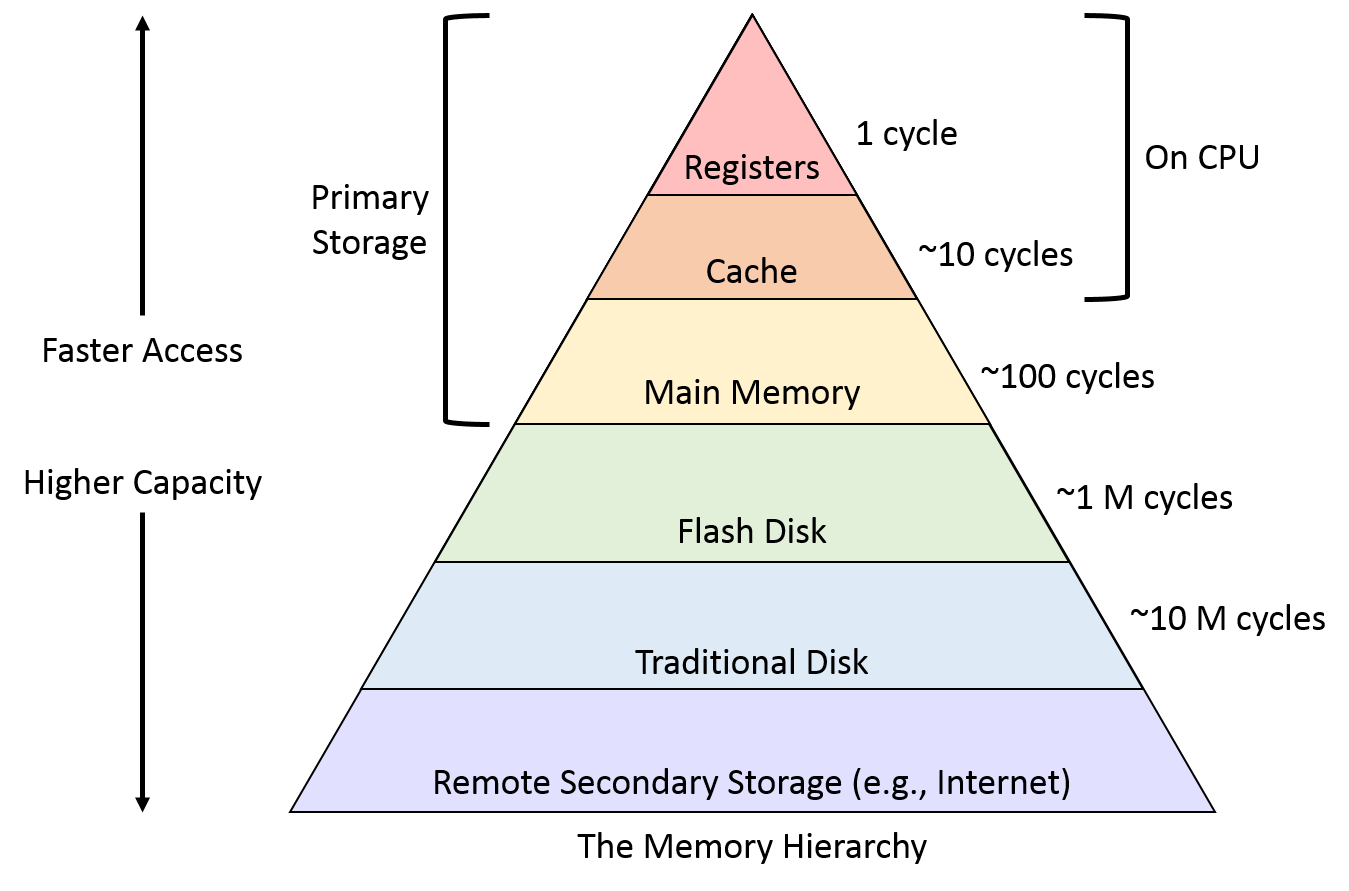
\includegraphics[width=1.0\textwidth]{figures/MemoryHerarchy.png}
    \label{fig:MemoryHerarchy}
  \end{figure}
\end{frame}

\begin{frame}{How does many values has singles variable?}
  \begin{itemize}
    \item One?
    \item Two?
  \end{itemize}
\end{frame}\begin{frame}{How does many values has singles variable?}
  \begin{itemize}
    \item One?
    \item Two?
  \end{itemize}
\end{frame}

\begin{frame}{A variable has two values}
  \begin{itemize}
    \item One : Its current value 
    \item Two : Its current addres
  \end{itemize}
\end{frame}

\subsection{Copy}
\begin{frame}[fragile]{Passing by Copy}
  \begin{itemize}
    \item When parameters are passed by copy, a new instance of the argument is created.
    \item Modifications within the function do not affect the original variable.
    \item Best used when you need to ensure the original data remains unchanged.
\end{itemize}

\begin{lstlisting}
  void incrementByCopy(int x) {
      x = x + 1;
      cout << "Inside function: " << x << endl;
  }
  
  int main() {
      int a = 5;
      incrementByCopy(a);
      cout << "Outside function: " << a << endl;
  }
  \end{lstlisting}

\end{frame}

\subsection{Reference}

\begin{frame}[fragile]{Passing by Reference}
  \begin{itemize}
    \item Passing by reference sends a reference to the original variable.
    \item Any changes inside the function affect the original variable.
    \item More efficient for large data structures but must be used carefully.
  \end{itemize}
  
  \begin{lstlisting}
  void incrementByReference(int& x) {
      x = x + 1;
      cout << "Inside function: " << x << endl;
  }
  
  int main() {
      int a = 5;
      incrementByReference(a);
      cout << "Outside function: " << a << endl;
  }
  \end{lstlisting}
\end{frame}

\begin{frame}
  \begin{figure}[h]
    \centering
    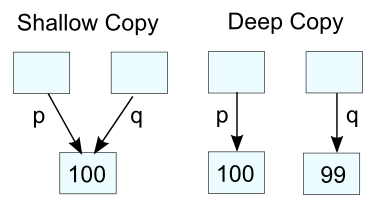
\includegraphics[width=1.0\textwidth]{figures/deep_vs_shallow_copy.png}
    \label{fig:MemoryHerarchy}
  \end{figure}
\end{frame}

\end{document}